\subsubsection{Systemkontext}
\label{sec:Kap-6.1.3.1}

IREB definiert den sogenannten Systemkontext als 

\vspace{1mm} %%% für Druck

\sttpzitat{„[den] Teil der Umgebung eines Systems, der für die Definition und das Verständnis der Anforderungen des betrachteten Systems relevant ist“. \cite[13]{poh15}}{}

\vspace{1mm} %%% für Druck

Bei der Bestimmung des Systemkontexts werden in der Umgebung des zu ent\-wickelnden Systems alle materiellen und immateriellen Aspekte identifiziert, die beim späteren Einsatz des Systems in irgendeiner Art und Weise mit ihm in Verbindung stehen werden. Dabei kann es sich um andere Software- oder Hardwaresysteme handeln, zu denen das zukünftige System Schnittstellen vorsehen muss. Zum System\-kontext gehören aber auch die Geschäftsprozesse, die das System unterstützen soll sowie rechtliche oder organisatorische Vorgaben (Gesetze, Richtlinien, Standards etc.), die beim Betrieb des Systems eingehalten werden müssen. Weiterhin gehören zum Systemkontext die verschiedenen Stakeholder. 

Die Bestimmung des Systemkontexts ist wichtig, um die Zusammenhänge zwischen dem zu entwickelnden System und seiner Umgebung zu verstehen bzw. vorzugeben. Dafür muss noch während der Entwicklung des Softwaresystems eine Annahme bzw. Festlegung darüber getroffen werden, wie sich das fertige System in seine Umgebung integrieren wird bzw. soll, um den Ausschnitt der Realwelt bestimmen zu können, der relevant für die zu ermittelnden Anforderungen an das System ist.

Falls Ihnen an dieser Stelle der schon bekannte (Kap. 3.2.2) Begriff der Domäne in den Sinn kommt, ist das kein Zufall. \marginline{Systemkontext und Domäne} Die \textbf{Domäne} ist der für das Softwareprodukt relevante Ausschnitt der Realwelt. Der \textbf{Systemkontext} ist der für die Anforderungen an das Softwareprodukt relevante Ausschnitt der Realwelt. Beide Begriffe beschreiben damit dasselbe Original: den relevanten Ausschnitt der Realwelt, allerdings mit unterschiedlichen Blickwinkeln. Der Blickwinkel des Begriffs Systemkontext ist enger, da er sich rein auf die Anforderungen fokussiert. Im Rahmen des Requirements Engineering wird fast ausschließlich der Begriff Systemkontext verwendet. Wenn Sie sich im Softwareengineering außerhalb des Requirements Engineering-Kontexts bewegen, finden Sie eher den Begriff Domäne.

\vspace{\baselineskip} %%% für Druck

\begin{figure}[h!]
	\centering
	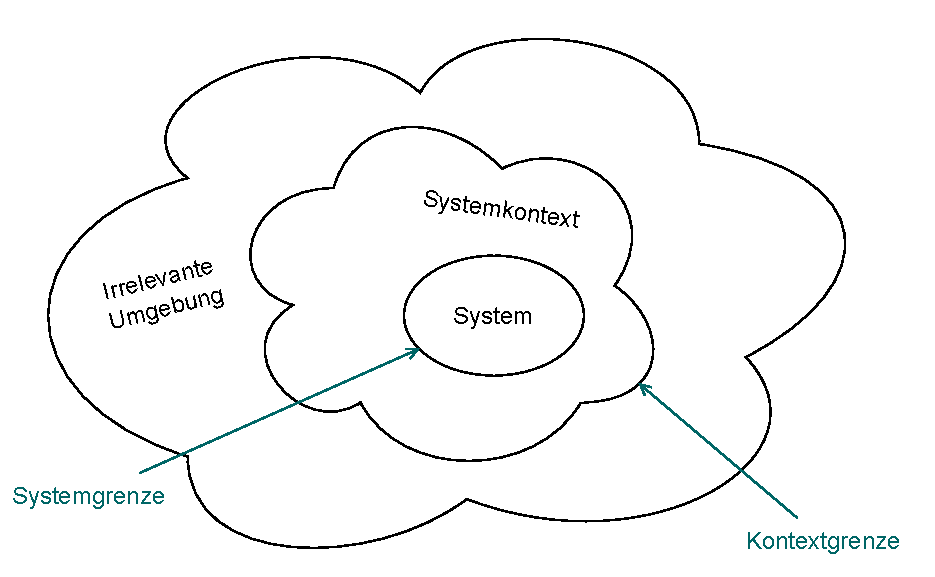
\includegraphics[scale=0.75]{Bilder/Kapitel-6/system-system.pdf}
	\caption[System, Systemkontext und irrelevante Umgebung]{System, Systemkontext und irrelevante Umgebung. Eigene Abbildung in Anlehnung an \cite[15]{poh15}}
	\label{fig:system-system}
\end{figure}

\vspace{\baselineskip} %%% für Druck

Die Grenze zwischen dem Softwaresystem und dem Systemkontext bezeichnet man als Systemgrenze. Abbildung~\ref{fig:system-system} zeigt in der Mitte das System (das zu entwickelnde Softwareprodukt) und getrennt durch die Systemgrenze es umgebend seinen System\-kontext. Die Außengrenze des Systemkontexts bildet die sogenannte Kontextgrenze. Diese trennt die relevante Umgebung des Systems (den Systemkontext) von der irrelevanten Umgebung des Systems. Aspekte, die (von der Mitte aus gesehen) außerhalb der Kontextgrenze liegen, haben keinen Einfluss auf den Entwicklungsprozess des Softwaresystems. Insbesondere erzeugen sie keine Anforderungen an das System.

Die Bestimmung des Systemkontexts ist eine wichtige Aufgabe in einem Softwareentwicklungsprojekt. Ein fehlerhaft oder unvollständig festgelegter Systemkontext wird meist erst beim Betrieb des fertigen Softwareprodukts auffallen und sich zum Beispiel durch fehlende Schnittstellen zu anderen Systemen, unzureichende Unterstützung vorhandener Geschäftsprozesse oder Nichtberücksichtigung der Wünsche einzelner Nutzergruppen äußern. Ein ungünstig festgelegter Systemkontext kann sich im Übrigen nicht nur durch \textbf{fehlende} Aspekte äußern, sondern auch darin, dass das neue System in Kontexten agiert, die schon durch vorhandene Systeme abgedeckt werden können. In solchen Fällen sind Ressourcen des Softwareentwicklungsprojekts womöglich unnötig eingesetzt worden.

Der \marginline{Systemkontext und An\-for\-derungs\-ermitt\-lung} Zeitpunkt der Festlegung des Systemkontexts in einem Softwareentwicklungsprojekt ist abhängig von der Art des eingesetzten Vorgehensmodells. Sequentielle Modelle bestimmen den Systemkontext üblicherweise während des Teilprozesses der Anforderungsermittlung. Die Ermittlung konkreter Anforderungen und die Bestimmung des Systemkontexts sind dabei eng verbunden. Eine komplett lineare Abfolge zwischen Bestimmung des Systemkontexts und Bestimmung der Anforderungen ist nicht realistisch. Gerade zu Beginn der Requirements Engineering-Phase werden Grauzonen in der Abgrenzung zwischen System und Systemkontext auf der einen Seite, aber auch zwischen Systemkontext und irrelevanter Umgebung auf der anderen Seite bestehen. Mit Abschluss der Requirements Engineering-Phase ist grundsätzlich auch die Festlegung des Systemkontexts abgeschlossen. Sollte die Änderung von Anforderungen im Softwareentwicklungsprojekt nach der Requirements Engineering-Phase aber möglich sein, kann sich auch der Systemkontext noch verändern. Bei konfigurierbaren Systemen, die für die Bedürfnisse verschiedener Nutzergruppen unterschiedlich angepasst werden können, kann sich die Systemgrenze zwischen den einzelnen konfigurierten Produktversionen unterscheiden.

Agile Modelle verzichten komplett darauf, den Systemkontext schon zu Beginn des Softwareentwicklungsprojekts abschließend festzulegen. Hier können sich in Abhängigkeit der Veränderung von Anforderungen Systemgrenze und Kontextgrenze mit jeder Iteration verschieben.

\vspace{2mm} %%% für Druck

\minisec{Dokumentation des Systemkontexts}

Für die Darstellung des Systemkontexts werden unterschiedliche Notationen in der Literatur vorgeschlagen. \marginline{Kom\-po\-nen\-ten\-diagramm} Aus dem Umfeld der UML-Diagramme könnte man das Komponentendiagramm verwenden, das Komponenten und ihre Schnittstellen darstellen kann. Das zu entwickelnde System könnte als eine Komponente und jedes Element des Systemkontexts als weitere Komponente modelliert werden. Der hauptsächliche Einsatzzweck eines UML-Komponentendiagramms ist allerdings die Modellierung von Softwarearchitekturen. Es wird üblicherweise im Prozess des Softwareentwurfs eingesetzt, um die Komponenten des zu entwickelnden Software\-systems und ihre Schnittstellen untereinander darzustellen. Insofern ist das Komponentendiagramm auf eine deutlich niedrigere Abstraktionsebene optimiert, als sie für die Darstellung des Systemkontexts benötigt wird und legt gleichzeitig den Fokus auf systeminterne Beziehungen anstatt auf die Beziehungen des Systems mit seiner 
\linebreak %%% für Druck
Umgebung.

Beziehungen des Systems mit seiner Außenwelt modelliert das UML-Anwen\-dungs\-fall\-diagramm, das daher auch ein potentieller Kandidat für die Darstellung des System\-kontexts ist. \marginline{An\-wen\-dungs\-fall\-diagramm} Es beschreibt, welche Anwendungsfälle mit dem System durchgeführt werden können, aber nicht auf welche Weise das System diese realisiert. Insofern bietet das Anwendungsfalldiagramm im Unterschied zum Komponenten\-diagramm das für die Darstellung des Systemkontexts gewünschte hohe Abstraktions\-niveau. Gleichzeitig ist die Syntax des UML-Anwendungsfalldiagramms auch für 
\linebreak %%% für Druck
IT-ferne Personen leicht erlernbar, sodass Anwendungsfalldiagramme sehr gut in Diskussionszusammenhängen mit den Kunden eingesetzt werden können. Zudem werden Anwendungsfalldiagramme häufig sowieso an anderer Stelle des Requirements Engineering eingesetzt. Genau dies spricht aber auch gegen das Anwendungsfall\-diagramm für die Darstellung des Systemkontexts, denn auch das Anwendungsfalldiagramm hat eigentlich andere Einsatzgebiete. In erster Linie wird ein Anwendungs\-fall\-diagramm verwendet, um auf einem sehr hohen Abstraktionsniveau die Interaktion der verschiedenen (menschlichen und nicht-menschlichen) Nutzergruppen mit dem System zu modellieren und ist damit ein Diagramm zur Darstellung von Verhalten. Die Verwendung eines Verhaltensdiagramms zur Darstellung des System\-kontexts, bei der man einen strukturellen Fokus einnimmt, ist nicht optimal.

\begin{figure}[h!]
	\centering
	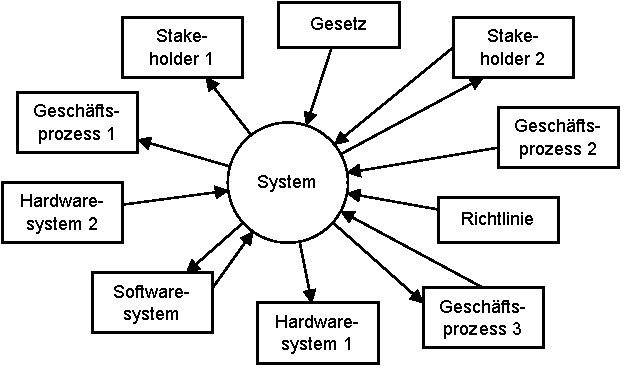
\includegraphics[scale=1.0]{Bilder/Kapitel-6/system.pdf}
	\caption{Kontextdiagramm der Strukturierten Analyse}
	\label{fig:kontextdiagramm_strukturierte_analyse}
\end{figure}

Außerhalb \marginline{Kontext\-diagramm} der Diagrammarten der UML existiert dagegen ein spezifisches Diagramm zur Darstellung des Systemkontexts, das sogenannte Kontextdiagramm der Strukturierten Analyse, die wir im historischen Überblick zur Entstehung des Software\-engineering in Abschnitt~1.1 kurz % TODO Referenz Abschnitt~\ref{sec:Kap-1.1}
angesprochen hatten. Als Bestandteil der Strukturierten Analyse gehört das Kontextdiagramm nicht zum Bereich der objektorientierten Softwareentwicklung, es ist nicht \textbf{Objekt}-orientiert, sondern \textbf{Datenfluss}-orientiert. Es wird, da es sehr bekannt ist -- aber sicher auch mangels anderer guter Alternativen -- auch in vielen objektorientierten Softwareentwicklungsprojekten eingesetzt. Abbildung~\ref{fig:kontextdiagramm_strukturierte_analyse} zeigt ein Kontextdiagramm.

Das System wird in der Mitte des Diagramms als Kreis dargestellt und ist von den Elementen des Systemkontexts (dargestellt als Rechtecke) umgeben. Die Pfeile zwischen dem System und den Elementen des Systemkontexts zeigen Datenflüsse in und aus dem System und symbolisieren so die zukünftigen Schnittstellen zwischen dem System und seiner Umgebung. Durch die sehr überschaubare Menge an Syntax\-elementen ist das Kontextdiagramm wie das UML-Anwendungsfalldiagramm auch für technisch nicht-versierte Kunden leicht verständlich. Gerade zu Beginn der Require\-ments Engineering-Tätigkeiten reicht es häufig, darzustellen, an welchen Stellen Schnittstellen zwischen dem zu entwickelnden System und dem System\-kontext berücksichtigt werden müssen, und nicht anzugeben, welche Informationen genau über diese Schnittstellen ausgetauscht werden sollen. Wie in Abbildung~\ref{fig:kontextdiagramm_strukturierte_analyse} sind dann die Pfeile nicht beschriftet und die Datenflüsse somit nicht näher spezifiziert. Bei konkreteren Beschreibungen des Systemkontexts und der Datenflüsse sollte man darauf achten, die Informationen, die zwischen dem System und Elementen des Systemkontexts ausgetauscht werden, nicht zu detailliert und nicht zu technisch darzustellen, um die einfache Lesbarkeit des Diagramms auch für die Kunden beizubehalten. 

\begin{itemize}[
	label={\sttpHervorhebung{$\Rightarrow$}},
	]
	\item Das UML-Komponentendiagramm sollte man eher nicht für die Darstellung des Systemkontexts verwenden. Das UML-Anwendungsfalldiagramm ist die geeignetste Diagrammart, wenn man das UML-Umfeld nicht verlassen möchte. Das Kontextdiagramm der Strukturierten Analyse kann man aufgrund seiner Einfachheit auch ohne Kenntnis der Methode der Strukturierten Analyse gut einsetzen. Ansonsten bleibt natürlich immer auch die Möglichkeit, sich mit einfachen Kästen und Pfeilen ein projektspezifisches Kontextdiagramm zu erstellen.
\end{itemize}